\begin{center}
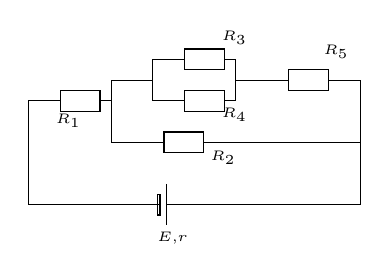
\begin{tikzpicture}[x=0.75pt,y=0.75pt,yscale=-1,xscale=1]
%uncomment if require: \path (0,300); %set diagram left start at 0, and has height of 300

%Shape: Battery [id:dp41038864580231404] 
\draw   (160,130) -- (173.5,130) (176.5,120) -- (176.5,140) (176.5,130) -- (190,130) (172.3,125) -- (173.5,125) -- (173.5,135) -- (172.3,135) -- (172.3,125) -- cycle ;
%Straight Lines [id:da3163365738659809] 
\draw    (190,130) -- (270,130) ;
%Straight Lines [id:da05173675712222314] 
\draw    (110,80) -- (110,130) ;
%Straight Lines [id:da47804297862757794] 
\draw    (110,80) -- (120,80) ;
%Straight Lines [id:da9057643206618209] 
\draw    (150,70) -- (150,100) ;
%Shape: Resistor [id:dp9965546099949054] 
\draw   (125.4,75) -- (144.6,75) -- (144.6,85) -- (125.4,85) -- (125.4,75) -- cycle (120,80) -- (125.4,80) (144.6,80) -- (150,80) ;
%Straight Lines [id:da0755765621865847] 
\draw    (170,60) -- (170,80) ;
%Straight Lines [id:da5506543591062112] 
\draw    (110,130) -- (160,130) ;
%Shape: Resistor [id:dp5943525570087891] 
\draw   (175.4,95) -- (194.6,95) -- (194.6,105) -- (175.4,105) -- (175.4,95) -- cycle (170,100) -- (175.4,100) (194.6,100) -- (200,100) ;
%Straight Lines [id:da20458298027628818] 
\draw    (150,100) -- (170,100) ;
%Straight Lines [id:da4442305975937406] 
\draw    (200,100) -- (270,100) ;
%Straight Lines [id:da35717809113951704] 
\draw    (150,70) -- (170,70) ;
%Straight Lines [id:da3625645367127812] 
\draw    (170,80) -- (180,80) ;
%Shape: Resistor [id:dp27044674641893796] 
\draw   (185.4,75) -- (204.6,75) -- (204.6,85) -- (185.4,85) -- (185.4,75) -- cycle (180,80) -- (185.4,80) (204.6,80) -- (210,80) ;
%Shape: Resistor [id:dp9888935439946336] 
\draw   (185.4,55) -- (204.6,55) -- (204.6,65) -- (185.4,65) -- (185.4,55) -- cycle (180,60) -- (185.4,60) (204.6,60) -- (210,60) ;
%Straight Lines [id:da2570097891204668] 
\draw    (170,60) -- (180,60) ;
%Straight Lines [id:da8597169745318671] 
\draw    (210,60) -- (210,80) ;
%Straight Lines [id:da6968281670670353] 
\draw    (210,70) -- (230,70) ;
%Shape: Resistor [id:dp9106011423679721] 
\draw   (235.4,65) -- (254.6,65) -- (254.6,75) -- (235.4,75) -- (235.4,65) -- cycle (230,70) -- (235.4,70) (254.6,70) -- (260,70) ;
%Straight Lines [id:da7437742845966437] 
\draw    (260,70) -- (270,70) ;
%Straight Lines [id:da46641133055265294] 
\draw    (270,70) -- (270,130) ;

% Text Node
\draw (171,142) node [anchor=north west][inner sep=0.75pt]  [font=\tiny] [align=left] {$\displaystyle \ms E$,$\displaystyle r$};
% Text Node
\draw (122,85) node [anchor=north west][inner sep=0.75pt]  [font=\tiny] [align=left] {$\displaystyle R_{1}$};
% Text Node
\draw (196.6,103) node [anchor=north west][inner sep=0.75pt]  [font=\tiny] [align=left] {$\displaystyle R_{2}$};
% Text Node
\draw (202,45) node [anchor=north west][inner sep=0.75pt]  [font=\tiny] [align=left] {$\displaystyle R_{3}$};
% Text Node
\draw (202,82) node [anchor=north west][inner sep=0.75pt]  [font=\tiny] [align=left] {$\displaystyle R_{4}$};
% Text Node
\draw (251,52) node [anchor=north west][inner sep=0.75pt]  [font=\tiny] [align=left] {$\displaystyle R_{5}$};


\end{tikzpicture}

\end{center}